%%\documentclass[a4paper,11pt]{article}
\documentclass[11pt]{article}

\usepackage[left=2.5cm, right=2cm, top=1.5cm, bottom=3cm]{geometry}
\usepackage[utf8]{inputenc}
\usepackage[T1]{fontenc}
\usepackage{titlesec}
\usepackage{enumitem}
\usepackage{graphicx}
\usepackage{amsmath}
\usepackage{amsfonts}
\usepackage{amssymb}
\usepackage{parskip}
\usepackage{float}
\usepackage{setspace}
\usepackage{fancyhdr}

\pagestyle{fancy}
\fancyhf{}
\setlength{\headheight}{65pt}
\setlength{\headsep}{24pt}
\fancyhead[L]{
\includegraphics[width=\textwidth]{picture/logoSW2026.pdf}}
\renewcommand{\headrulewidth}{0pt}
\fancyfoot[C]{\thepage}
\setlength{\footskip}{14pt}

\setstretch{1.12}
\setlength{\parskip}{0.65em}
\setlist[itemize]{leftmargin=1.35cm, itemsep=0.45em, topsep=0.35em}
\setlist[enumerate]{leftmargin=1.35cm, itemsep=0.45em, topsep=0.35em}

\titleformat{\section}{\normalfont\Large\bfseries}{\thesection}{1em}{}
\titleformat{\subsection}{\normalfont\large\bfseries}{\thesubsection}{1em}{}

\title{Informe del Proyecto}

\begin{document}

\renewcommand{\thesection}{\Roman{section}}
\begin{center}
    \textbf{\underline{\normalsize APE 1}}
\end{center}

\section{PORTADA}

\begin{tabbing}
    \textbf{Tema:}\hspace{1cm} \= Ecualizador para procesamiento de imágenes \\[0.25em]
    \textbf{Carrera:}\hspace{1cm} \= Ingeniería de Software \\[0.25em]
    \textbf{Unidad de Organización Curricular:} \hspace{1cm} \= PROFESIONAL \\[0.25em]
    \textbf{Nivel y Paralelo:} \> Séptimo semestre A \\[0.25em]
    \textbf{Alumnos participantes:} \> Bonilla Guerrero Fernando Joel \\
    \> García Abata Josué Joel \\[0.25em]
    \textbf{Asignatura:} \> Gestión de Proyectos \\[0.25em]
    \textbf{Docente:} \> Ing. Rubén Nogales, Mg.
\end{tabbing}

\section{INFORME DE GUÍA PRÁCTICA}
\renewcommand{\thesection}{\arabic{section}}

\subsection{Objetivos}
\textbf{General:}
\begin{itemize}
    \item Aplicar un flujo de procesamiento sobre una imagen de retina para mejorar la visualización de detalles poco evidentes a simple vista mediante normalización por canales RGB, compresión en escala de grises y binarización por umbral.
\end{itemize}

\textbf{Específicos:}
\begin{itemize}
    \item Analizar la distribución de intensidades de la imagen original mediante sus histogramas por canal R, G y B antes y después de aplicar la normalización.
    \item Aplicar la normalización min-max por canal para ampliar el contraste de la imagen y resaltar estructuras como posibles exudados que no se aprecian en la imagen original.
    \item Obtener la imagen comprimida en escala de grises y su versión binaria, observando el efecto de los controles de tamaño de bloque y umbral en el resultado final.
\end{itemize}

\subsection{Modalidad}
\begin{tabbing}
    \hspace{1cm} \= Presencial.
\end{tabbing}

\subsection{Tiempo de duración}
\begin{tabbing}
    \hspace{1cm} \= \textbf{Presenciales:} \= 8 \\
    \hspace{1cm} \= \textbf{No presenciales:} \= 0
\end{tabbing}

\subsection{Instrucciones}
\begin{enumerate}
    \item Seleccionar una imagen de entrada para realizar el procesamiento.
    \item Normalizar la imagen y observar los cambios generados en su representación visual.
    \item Visualizar la imagen desde sus canales de color para comparar la información presente en cada uno.
    \item Comprimir la imagen en escala de grises mediante bloques de reducción.
    \item Aplicar binarización por umbral para obtener una imagen compuesta únicamente por valores claros y oscuros.
\end{enumerate}

\subsection{Listado de equipos, materiales y recursos}
Listado de equipos y materiales generales empleados en la guía práctica:
\begin{itemize}
    \item Computador.
    \item Imagen de prueba relacionada con una retina.
    \item Herramienta de procesamiento de imágenes.
    \item Internet.
\end{itemize}

\textbf{TAC (Tecnologías para el Aprendizaje y Conocimiento) empleados en la guía práctica:}

$\square$ Plataformas educativas \\
$\square$ Simuladores y laboratorios virtuales \\
$\blacksquare$ Aplicaciones educativas \\
$\square$ Recursos audiovisuales \\
$\square$ Gamificación \\
$\square$ Inteligencia Artificial \\
Otros (Especifique): \underline{\hspace{5cm}}

\subsubsection{Librerías utilizadas}
Las siguientes librerías externas de Python fueron empleadas en el desarrollo de la aplicación:

\begin{table}[H]
    \centering
    \begin{tabular}{|l|l|p{7cm}|}
        \hline
        \textbf{Librería}      & \textbf{Versión mínima} & \textbf{Propósito}                                                               \\
        \hline
        \texttt{numpy}         & 1.24                    & Operaciones matriciales y manipulación de arreglos de píxeles.                   \\
        \hline
        \texttt{opencv-python} & 4.7                     & Lectura de imágenes, conversión de espacios de color y procesamiento de canales. \\
        \hline
        \texttt{Pillow}        & 9.0                     & Conversión de imágenes para su visualización en la interfaz gráfica.             \\
        \hline
        \texttt{matplotlib}    & 3.6                     & Generación de histogramas por canal y figuras embebidas en la interfaz.          \\
        \hline
        \texttt{customtkinter} & 5.0                     & Construcción de la interfaz gráfica con componentes modernos sobre Tkinter.      \\
        \hline
    \end{tabular}
    \caption{Librerías externas utilizadas en la aplicación.}
\end{table}

\subsubsection{Acceso a la aplicación}
Para ejecutar la aplicación, se requiere Python 3.10 o superior con las librerías listadas instaladas. El punto de entrada es el archivo \texttt{app.py}, ubicado en la raíz del proyecto. Los pasos son los siguientes:

\begin{enumerate}
    \item Instalar las dependencias ejecutando en terminal:\\
          \texttt{pip install numpy opencv-python Pillow matplotlib customtkinter}
    \item Ejecutar la aplicación:\\
          \texttt{python app.py}
\end{enumerate}

\subsection{Actividades por desarrollar}
\begin{enumerate}
    \item Cargar la imagen de retina y generar los histogramas originales por canal.
    \item Aplicar la normalización por canal y generar los histogramas normalizados.
    \item Obtener la imagen en escala de grises, comprimirla por bloques y aplicar la binarización por umbral.
    \item Comparar la imagen original, la normalizada y la comprimida en escala de grises.
\end{enumerate}

\subsection{Resultados obtenidos}

En esta sección se documenta el procedimiento aplicado sobre una única imagen de retina. Se parte de la imagen original, se analizan sus histogramas por canal, se aplica la normalización, se obtiene la imagen normalizada junto con su versión en escala de grises y binaria, y finalmente se comparan los resultados obtenidos.

\subsubsection{Imagen original utilizada}

La imagen empleada corresponde a una retinografía de fondo de ojo, presentada tal como fue capturada, sin modificación alguna. Esta imagen constituye el punto de partida del procesamiento y presenta un contraste reducido en varias zonas, lo que provoca que ciertos detalles del tejido retinal no se aprecien con facilidad a simple vista. Los posibles exudados duros, asociados a la retinopatía diabética, no se distinguen con claridad en la imagen sin procesar debido a su pequeño tamaño y a la baja diferencia de brillo respecto al tejido circundante.

Partir de una imagen con estas características resulta adecuado, ya que cualquier mejora del contraste aplicada sobre ella se traduce directamente en una mayor visibilidad de las estructuras que antes no eran evidentes, permitiendo observar el efecto real del procesamiento.

\begin{figure}[H]
    \centering
    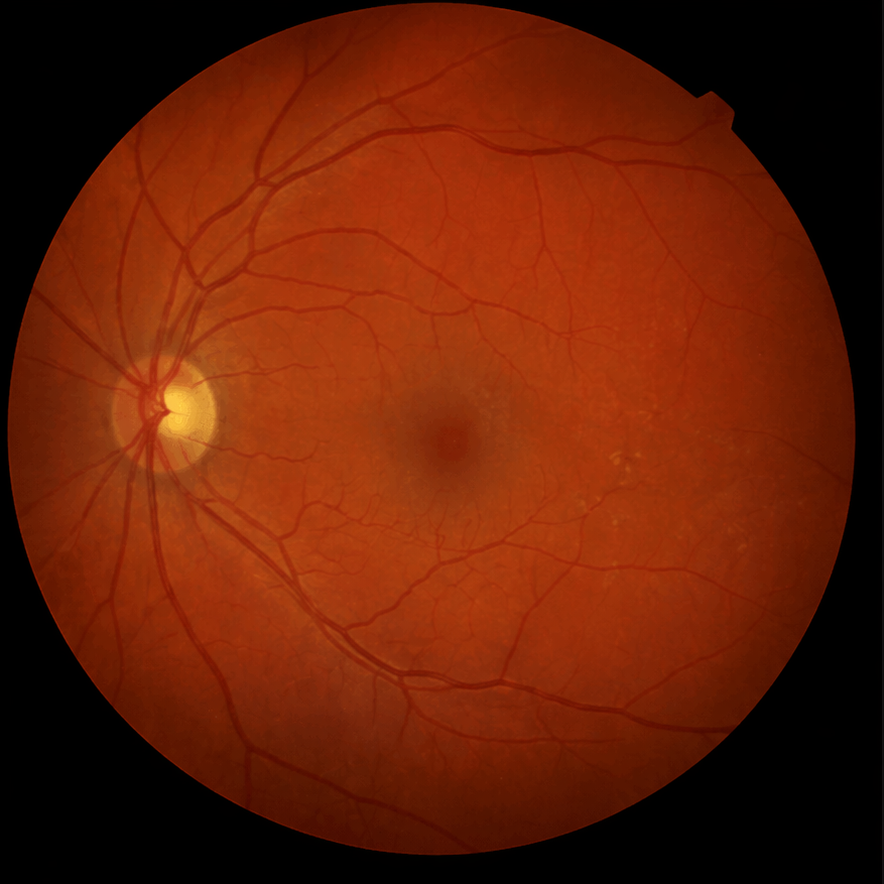
\includegraphics[width=0.55\textwidth]{picture/retina_correcion/retina_normal_diabetes.png}
    \caption{Imagen original de retina empleada como punto de partida del procesamiento.}
    \label{fig:retina_original}
\end{figure}

\subsubsection{Análisis de histogramas originales}

Antes de aplicar cualquier transformación, se generaron los histogramas de los tres canales RGB de la imagen original. Estos histogramas no representan ninguna modificación de la imagen; muestran la distribución real de intensidades de cada canal tal como aparece en la imagen base. El eje horizontal representa el valor de intensidad del píxel (de 0 a 255) y el eje vertical representa la cantidad de píxeles con ese valor.

\begin{figure}[H]
    \centering
    \begin{minipage}[t]{0.32\textwidth}
        \centering
        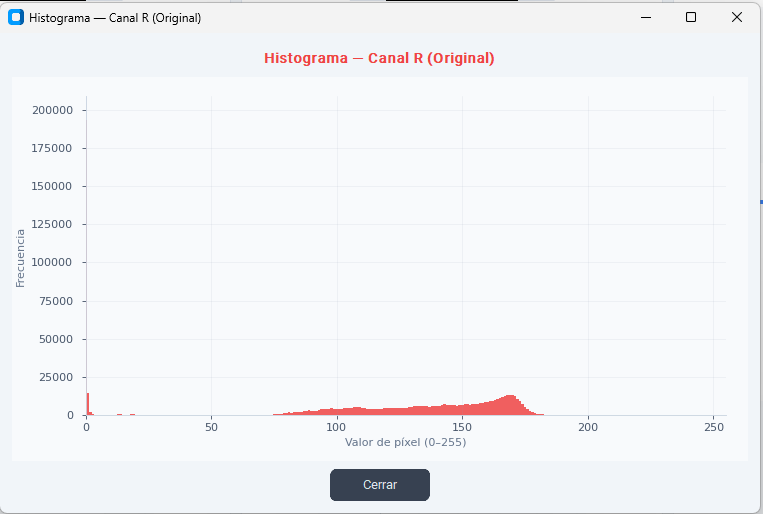
\includegraphics[width=\textwidth]{picture/retina_correcion/histograma_normal_rojo.png}
        \\[3pt]\small (a) Canal R original
    \end{minipage}
    \hfill
    \begin{minipage}[t]{0.32\textwidth}
        \centering
        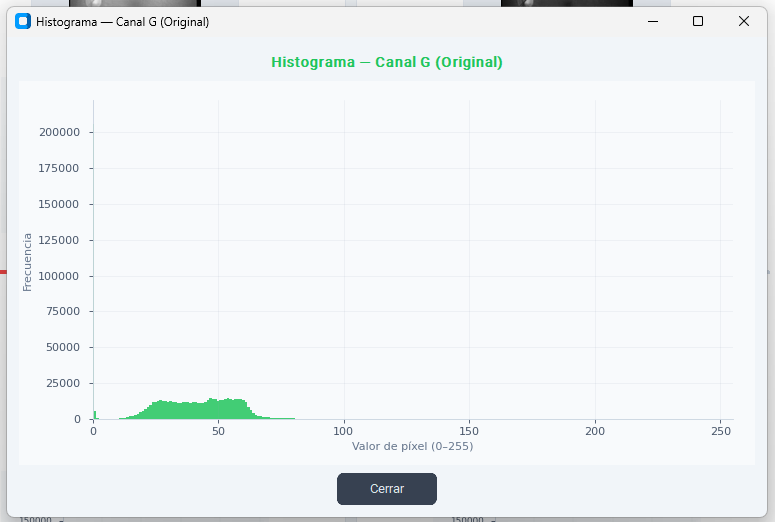
\includegraphics[width=\textwidth]{picture/retina_correcion/histograma_normal_verde.png}
        \\[3pt]\small (b) Canal G original
    \end{minipage}
    \hfill
    \begin{minipage}[t]{0.32\textwidth}
        \centering
        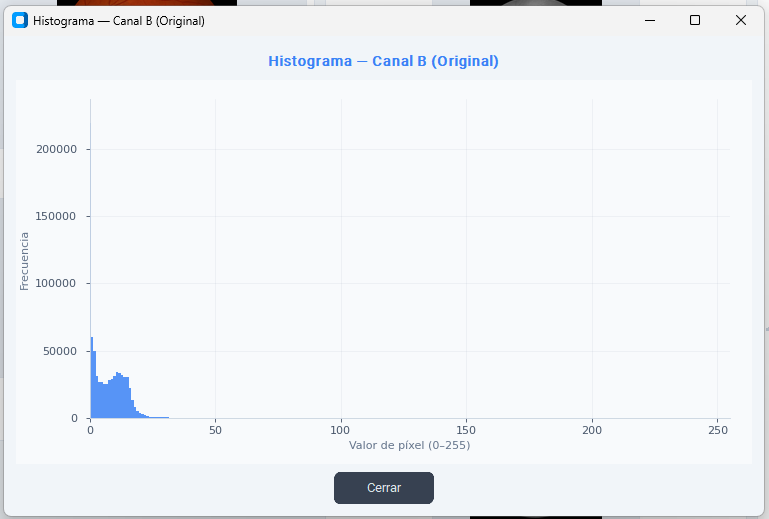
\includegraphics[width=\textwidth]{picture/retina_correcion/histograma_normal_azul.png}
        \\[3pt]\small (c) Canal B original
    \end{minipage}
    \caption{Histogramas originales de los canales R, G y B de la imagen de retina, sin procesamiento aplicado.}
    \label{fig:hist_orig}
\end{figure}

\textbf{Canal rojo.} El histograma muestra que gran parte de los valores se concentra aproximadamente entre 100 y 150. Esta concentración indica que el canal rojo contiene una intensidad predominante medio-alta, característica habitual en imágenes de retina debido a la coloración anaranjada-rojiza del tejido retinal y a la dispersión interna de la luz roja dentro del ojo. Al tratarse de la componente cromática dominante, el canal rojo aporta información sobre la iluminación general de la retina, pero el hecho de que la mayor parte de sus píxeles esté agrupada en un rango estrecho reduce las diferencias de brillo entre estructuras.

\textbf{Canal verde.} El histograma del canal verde presenta su actividad concentrada en un rango más estrecho, ubicado en intensidades bajas-medias. Esta concentración implica que la información útil del canal vive en una franja reducida del eje de intensidades. En imágenes de retina, esto ocurre porque la hemoglobina de los vasos absorbe la luz verde y el tejido circundante la refleja, generando una diferencia interna entre vasos y fondo dentro de ese rango acotado. Esta separación interna es la que convierte al canal verde en el más relevante para observar estructuras finas.

\textbf{Canal azul.} El histograma del canal azul muestra una distribución comprimida en valores bajos, con poca actividad a lo largo del eje. Esto se debe a que la luz azul es absorbida con rapidez por las capas superficiales del ojo y no alcanza las estructuras internas de la retina. Como resultado, la información en este canal es limitada y suele estar asociada a mayor ruido visual.

\subsubsection{Normalización por canales}

La normalización por canal es una técnica de preprocesamiento que redistribuye los valores de intensidad dentro de un rango específico elegido manualmente, llevándolo a ocupar el espacio completo de 0 a 255. Su utilidad concreta consiste en que, si la información útil de un canal se concentra en un rango estrecho, al estirar ese rango se amplían las diferencias de brillo entre estructuras y se mejora el contraste visual \cite{b1}.

La fórmula aplicada corresponde a la normalización min-max:
\begin{equation}
    p_{nuevo} = \frac{p - p_{\min}}{p_{\max} - p_{\min}} \times 255
    \label{eq:normalizacion}
\end{equation}
donde $p$ es el valor original del píxel, $p_{\min}$ y $p_{\max}$ son los límites inferior y superior del rango elegido, y $p_{nuevo}$ es el valor resultante. Los píxeles por debajo de $p_{\min}$ se fijan en 0 y los que superan $p_{\max}$ se fijan en 255. El valor $p_{\min}$ representa el umbral inferior a partir del cual se considera información útil, mientras que $p_{\max}$ representa el umbral superior por encima del cual se descartan valores saturados o fuera de interés.

Los rangos aplicados a cada canal son los siguientes:

\textbf{Canal rojo: $p_{\min} = 16$, $p_{\max} = 181$.} Este canal cuenta con un rango más amplio en el histograma original y contiene una parte importante de la información estructural general de la retina, relacionada con la iluminación global. Sin embargo, no es el canal donde se distinguen mejor los exudados, ya que su amplia penetración dentro del tejido tiende a suavizar los detalles finos. El rango seleccionado excluye el fondo negro y la saturación extrema, conservando la zona donde reside la información retinal efectiva.

\textbf{Canal verde: $p_{\min} = 34$, $p_{\max} = 72$.} Los valores útiles del canal verde se concentran entre 34 y 72, una franja estrecha de apenas 38 niveles. Al expandir ese rango a 0--255 mediante la ecuación~\eqref{eq:normalizacion}, se obtiene una amplificación notable del contraste: las pequeñas diferencias de intensidad entre los vasos, las lesiones y el tejido circundante se vuelven más grandes. Por esta razón, el canal verde es el más importante en el análisis de imágenes de retina, dado que ofrece el mejor contraste para observar vasos, bordes y alteraciones pequeñas como los posibles exudados.

\textbf{Canal azul: $p_{\min} = 8$, $p_{\max} = 68$.} El rango del canal azul es reducido porque su información original es limitada. El estiramiento de un rango tan pequeño distribuye la poca información útil con más espacio, pero no crea información nueva. El canal azul suele aportar menor utilidad diagnóstica en este tipo de análisis, ya que presenta menor definición visual y mayor ruido.

\subsubsection{Histogramas normalizados}

Tras aplicar la normalización se generaron los histogramas correspondientes a cada canal. Estos histogramas permiten verificar cómo cambia la distribución de intensidades después del procesamiento.

\begin{figure}[H]
    \centering
    \begin{minipage}[t]{0.32\textwidth}
        \centering
        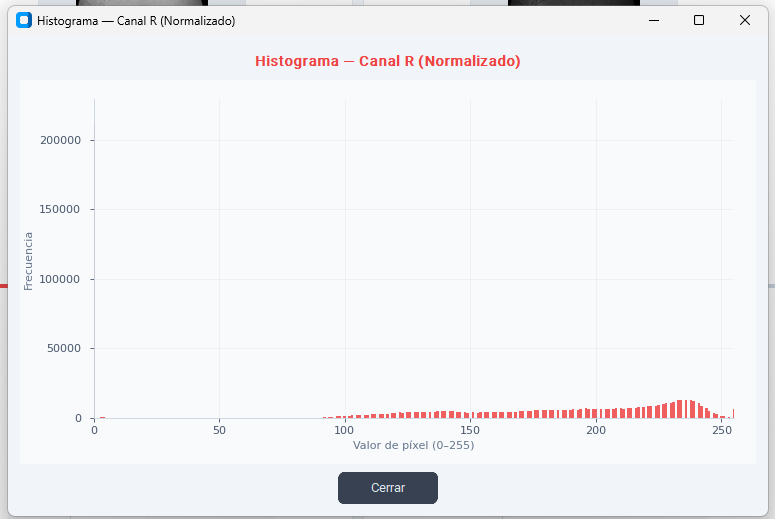
\includegraphics[width=\textwidth]{picture/retina_correcion/histograma_normalizado_rojo.png}
        \\[3pt]\small (a) Canal R normalizado
    \end{minipage}
    \hfill
    \begin{minipage}[t]{0.32\textwidth}
        \centering
        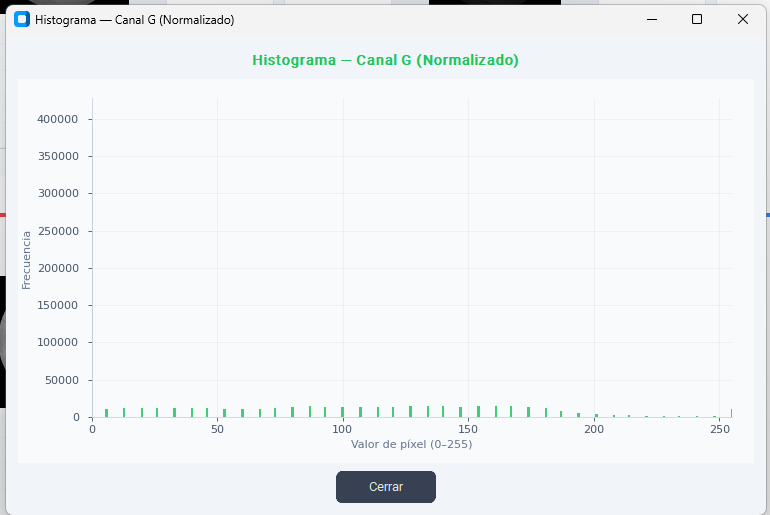
\includegraphics[width=\textwidth]{picture/retina_correcion/histograma_normalizado_verde.png}
        \\[3pt]\small (b) Canal G normalizado
    \end{minipage}
    \hfill
    \begin{minipage}[t]{0.32\textwidth}
        \centering
        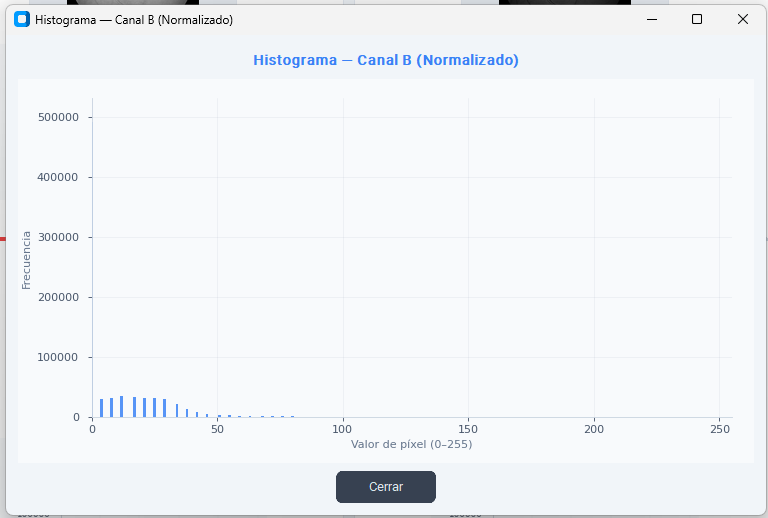
\includegraphics[width=\textwidth]{picture/retina_correcion/histograma_normalizado_azul.png}
        \\[3pt]\small (c) Canal B normalizado
    \end{minipage}
    \caption{Histogramas de los canales R, G y B tras aplicar la normalización min-max.}
    \label{fig:hist_norm}
\end{figure}

En los tres canales se observa que la distribución se expande y ocupa un tramo más amplio del eje de intensidades respecto al histograma original. Los valores inferiores al umbral mínimo se acumulan en el extremo izquierdo (valor 0) y los superiores al máximo en el extremo derecho (valor 255). La distribución intermedia, que en el original estaba comprimida, queda ahora repartida a lo largo de un rango mayor. Esto se traduce en mayores diferencias de brillo entre píxeles vecinos, lo cual es el mecanismo directo por el cual la normalización mejora el contraste percibido de la imagen.

\subsubsection{Comparación entre imagen original y normalizada}

La comparación lado a lado entre la imagen original y la imagen normalizada evidencia el efecto del procesamiento aplicado.

\begin{figure}[H]
    \centering
    \begin{minipage}[t]{0.46\textwidth}
        \centering
        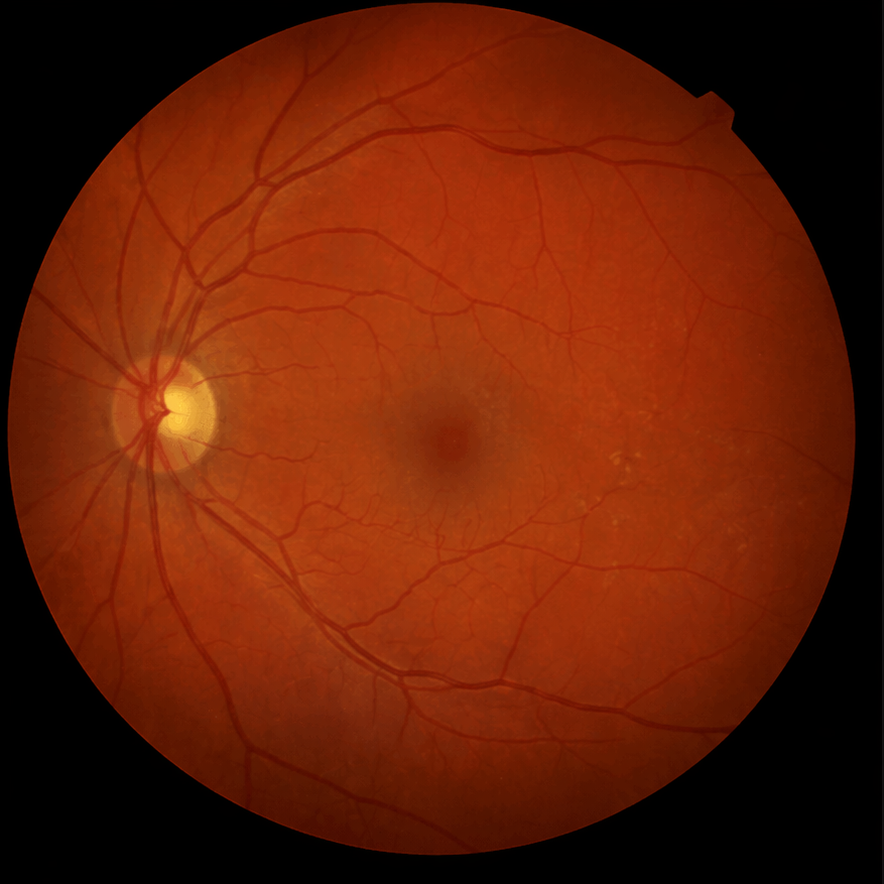
\includegraphics[width=\textwidth]{picture/retina_correcion/retina_normal_diabetes.png}
        \\[3pt]\small (a) Imagen original
    \end{minipage}
    \hfill
    \begin{minipage}[t]{0.46\textwidth}
        \centering
        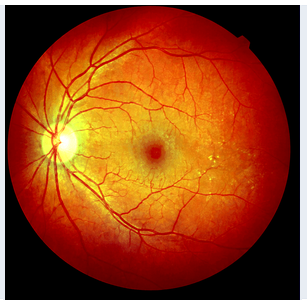
\includegraphics[width=\textwidth]{picture/retina_correcion/retina_normalizada.png}
        \\[3pt]\small (b) Imagen normalizada
    \end{minipage}
    \caption{Comparación entre la imagen original y la imagen tras aplicar la normalización por canales.}
    \label{fig:comparacion_norm}
\end{figure}

La imagen original se observa apagada y con poco contraste en ciertas zonas, lo que impide distinguir los exudados a simple vista. Tras la normalización, la imagen gana contraste y los detalles del tejido retinal se vuelven más visibles, de modo que los exudados se aprecian con claridad. La normalización no crea lesiones ni agrega información nueva a la imagen: redistribuye las intensidades de color para que la información que ya estaba presente pase a ser perceptible visualmente.

Al inspeccionar la imagen normalizada, se identifican los exudados como manchas de coloración amarillenta distribuidas sobre el tejido retinal. La Figura~\ref{fig:exudados_marcados_color} muestra la ubicación de estos hallazgos marcados sobre la imagen normalizada.

\begin{figure}[H]
    \centering
    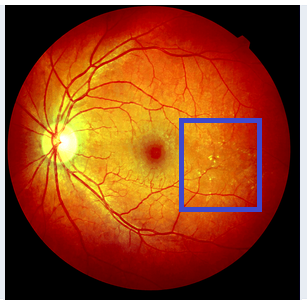
\includegraphics[width=0.6\textwidth]{picture/retina_correcion/retina_normalizada_exudados_marcados.png}
    \caption{Exudados identificados en la imagen normalizada.}
    \label{fig:exudados_marcados_color}
\end{figure}

\subsubsection{Análisis de canales Rojo, Verde y Azul}

Una vez observada la mejora general de la imagen tras la normalización, corresponde analizar qué aporta cada canal de color a esa mejora visual y, particularmente, cuál de ellos permite que los exudados resulten más distinguibles del tejido circundante. Cada canal aporta un tipo de información diferente según la manera en que la luz interactúa con los tejidos del ojo.

\textbf{Canal rojo.} La luz roja, de longitud de onda larga, penetra en profundidad dentro del tejido retinal y se dispersa ampliamente, iluminando extensas áreas de forma uniforme. Esto produce que el canal rojo muestre gran parte de la iluminación general de la retina, pero también que tienda a saturar zonas brillantes (como el disco óptico) y a suavizar los detalles finos. Su utilidad para identificar lesiones pequeñas es limitada.

\textbf{Canal verde.} La luz verde presenta el mejor equilibrio óptico en tejido retinal: penetra lo suficiente para capturar estructuras internas y es absorbida de forma diferenciada por la hemoglobina. Los vasos sanguíneos aparecen más oscuros y el tejido circundante más claro, generando un contraste local que facilita observar vasos, bordes y lesiones pequeñas como los exudados. Por esta razón, el canal verde es el referente estándar en el procesamiento de imágenes de retina \cite{b3}.

\textbf{Canal azul.} La luz azul, de longitud de onda corta, es absorbida por las capas superficiales del ojo y no alcanza las estructuras internas de la retina. El canal azul aporta menos información útil para este tipo de análisis, presenta menor claridad visual y mayor ruido, por lo que su aporte diagnóstico es reducido.

\subsubsection{Compresión, escala de grises y binarización}

Tras haber mejorado la visualización mediante la normalización y comprendido el aporte particular de cada canal de color, el siguiente paso consiste en simplificar la imagen para observar cómo se conservan o resaltan ciertos rasgos visuales al reducir la información de color y aplicar una binarización. Esta etapa entrega tres resultados visuales que se analizan a continuación.

\begin{figure}[H]
    \centering
    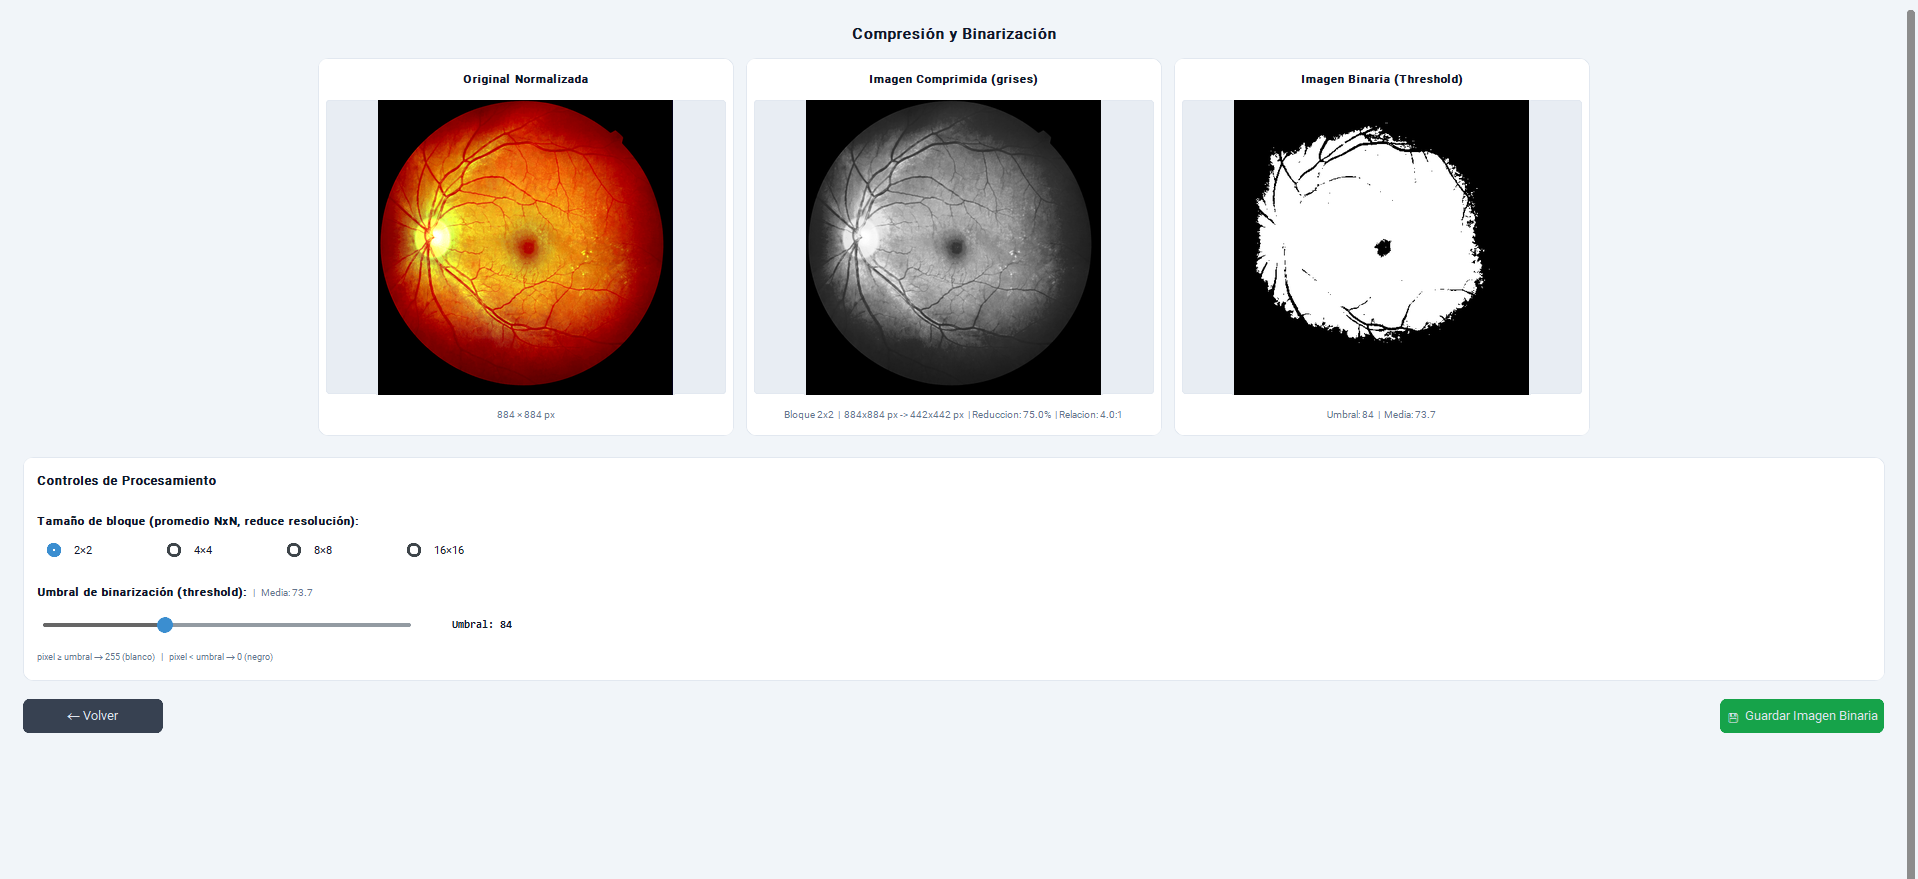
\includegraphics[width=0.9\textwidth]{picture/retina_correcion/imagen_retina_normalizacion_comprension_binario.png}
    \caption{Resultados de la segunda etapa: imagen normalizada, imagen comprimida en escala de grises e imagen binaria.}
    \label{fig:etapa_grises_binario}
\end{figure}

\textbf{Imagen normalizada.} Conserva los tres canales RGB y presenta una distribución de intensidades más amplia que la imagen original. Esta mejor distribución permite observar con mayor claridad los detalles del tejido retinal, incluidos los exudados, por lo que constituye la referencia con la que se comparan las transformaciones posteriores.

\textbf{Imagen comprimida en escala de grises.} Reduce la información de color a una única representación de intensidad, aplicando la ponderación estándar:
\begin{equation}
    I_{gris} = 0.299 \cdot R + 0.587 \cdot G + 0.114 \cdot B
    \label{eq:grises}
\end{equation}
El resultado descarta el color y conserva la información de brillo, lo que facilita la observación de zonas claras y oscuras, bordes y manchas presentes en la imagen \cite{b2}. En esta representación, los exudados duros aparecen como regiones de alta intensidad (blancas o muy claras), dado que son depósitos lipídicos que reflejan la luz con mayor intensidad que el tejido circundante. Los vasos sanguíneos, en cambio, absorben mayor cantidad de luz y presentan menor reflectancia, por lo que se representan como estructuras oscuras sobre el tejido de fondo. Sobre esta representación se aplica además una compresión por bloques, que agrupa los píxeles en regiones de tamaño $N \times N$ y las reemplaza por su valor promedio, reduciendo la cantidad total de datos mientras se mantienen los rasgos generales de la retina.

\textbf{Imagen binaria.} Transforma la imagen en escala de grises en una representación con solo dos valores principales, blanco y negro, aplicando un umbral $T$: los píxeles con intensidad mayor o igual al umbral se convierten en blanco y el resto en negro. Esta representación aporta una separación directa entre regiones claras y oscuras, lo que permite aislar zonas de mayor brillo asociadas a los exudados. Su principal limitación consiste en que depende por completo del umbral seleccionado, de modo que un valor mal ajustado puede producir falsos positivos, incluir ruido o eliminar detalles relevantes \cite{b4}.

\subsubsection{Controles de procesamiento}

El ecualizador dispone de dos controles que influyen directamente sobre el resultado final del procesamiento: el tamaño de bloque, que regula el nivel de simplificación aplicado a la imagen, y el umbral de binarización, que regula la separación entre regiones claras y oscuras. Ajustar estos parámetros con criterio es determinante para preservar los rasgos visuales relevantes.

\textbf{Tamaño de bloque.} Este control define el tamaño de la región cuadrada que se promedia en la compresión, de modo que cada grupo de $N \times N$ píxeles se reemplaza por un único valor. Su aporte consiste en reducir la resolución espacial de la imagen, disminuir el ruido local y rebajar la cantidad de datos a procesar; a cambio, se produce una pérdida progresiva de detalle fino. Según el tamaño seleccionado, el comportamiento es el siguiente:
\begin{itemize}
    \item \textbf{$2 \times 2$:} conserva la mayor parte del detalle. La simplificación es ligera y las estructuras finas, como bordes de vasos y pequeños exudados, se mantienen visibles.
    \item \textbf{$4 \times 4$:} reduce más información y permite una simplificación intermedia. La imagen conserva una representación aceptable, aunque comienzan a difuminarse los detalles más pequeños.
    \item \textbf{$8 \times 8$:} simplifica la imagen en mayor medida y resulta útil para observar patrones generales de iluminación, pero los elementos pequeños pierden nitidez.
    \item \textbf{$16 \times 16$:} reduce en exceso la información fina y puede ocultar lesiones pequeñas, por lo que resulta poco adecuado cuando se busca conservar exudados u otras estructuras de tamaño reducido.
\end{itemize}
El tamaño de bloque debe seleccionarse en función del objetivo del análisis: valores pequeños cuando se busca preservar el detalle y valores mayores cuando interesa observar patrones generales o reducir el volumen de datos.

Para evidenciar el efecto del tamaño de bloque sobre el resultado guardado, la Figura~\ref{fig:comparacion_peso} compara la imagen original con la imagen binaria obtenida tras aplicar compresión por bloques.

\begin{figure}[H]
    \centering
    \begin{minipage}[t]{0.46\textwidth}
        \centering
        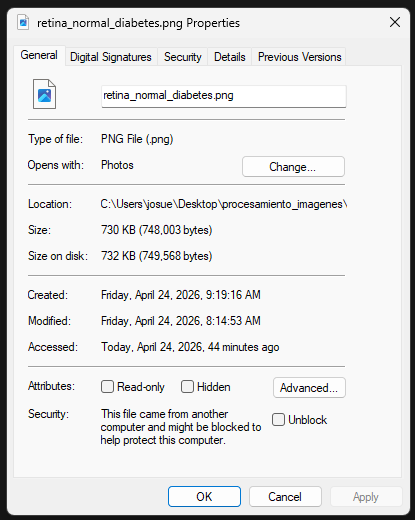
\includegraphics[width=\textwidth]{picture/retina_correcion/imagen_original_peso.png}
        \\[3pt]\small (a) Imagen original
    \end{minipage}
    \hfill
    \begin{minipage}[t]{0.46\textwidth}
        \centering
        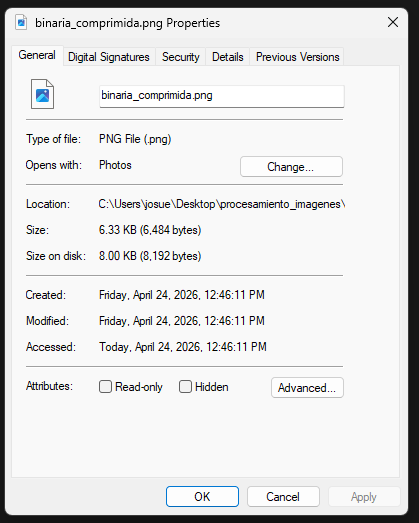
\includegraphics[width=\textwidth]{picture/retina_correcion/compresion_imagen_binaria.png}
        \\[3pt]\small (b) Imagen binaria comprimida
    \end{minipage}
    \caption{Comparación entre la imagen original y la imagen binaria resultante tras la compresión por bloques.}
    \label{fig:comparacion_peso}
\end{figure}

En este caso, se aplicó una compresión por bloques de $2 \times 2$, lo que implica que cada grupo de cuatro píxeles de la imagen original se reduce a un único valor representativo. Sobre esa imagen reducida se aplica posteriormente la binarización, cuyo resultado se almacena como salida final del procesamiento. La elección del tamaño $2 \times 2$ responde a una compresión moderada: el peso de la imagen disminuye sin que los detalles visuales relevantes se vean afectados, manteniendo visibles los bordes, las manchas pequeñas y los rasgos asociados a los exudados. Un tamaño superior, como $16 \times 16$, produciría una reducción mucho más agresiva, pero a costa de eliminar información importante para el análisis posterior, por lo que no resulta adecuado en este contexto.

La compresión cumple un papel relevante dentro de un flujo de procesamiento de imágenes, ya que reduce la cantidad de datos a procesar, facilita el almacenamiento de los resultados intermedios y genera representaciones que pueden emplearse como entrada de procesos posteriores como segmentación, extracción de características, análisis de objetos o clasificación. En particular, la imagen binaria obtenida aquí simplifica la información visual a dos niveles y permite distinguir con rapidez las regiones claras de las oscuras, lo que la convierte en una representación adecuada para etapas de análisis subsiguientes.

\textbf{Umbral de binarización.} Este control establece el valor límite de intensidad que separa las regiones claras de las oscuras durante la binarización. Los píxeles con valor igual o superior al umbral se representan como blancos y los inferiores como negros, por lo que su aporte consiste en definir qué zonas de la imagen se consideran relevantes frente al fondo. Un umbral alto restringe la selección únicamente a las zonas más brillantes, lo que puede aislar los exudados pero también eliminar regiones útiles. Un umbral bajo amplía la selección, lo que puede recuperar más detalle pero también introducir ruido y falsos positivos. El valor adecuado depende de las intensidades presentes en la imagen en escala de grises y suele requerir un ajuste iterativo hasta lograr una segmentación coherente con lo observado.

Para ilustrar el efecto directo del umbral sobre el resultado, la Figura~\ref{fig:comparacion_umbrales} presenta dos binarizaciones de la misma imagen utilizando umbrales distintos.

\begin{figure}[H]
    \centering
    \begin{minipage}[t]{0.46\textwidth}
        \centering
        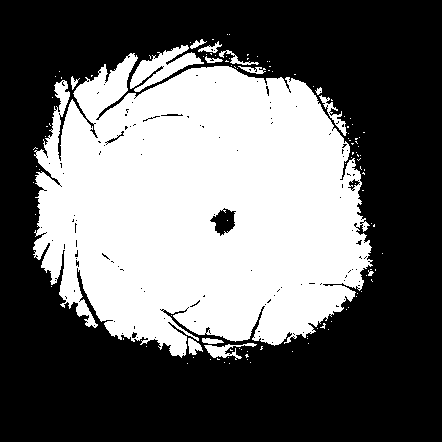
\includegraphics[width=\textwidth]{picture/retina_correcion/binaria_imagen_84.png}
        \\[3pt]\small (a) Binarización con umbral $T = 84$
    \end{minipage}
    \hfill
    \begin{minipage}[t]{0.46\textwidth}
        \centering
        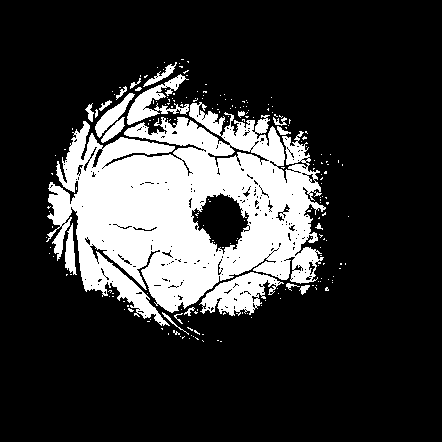
\includegraphics[width=\textwidth]{picture/retina_correcion/imagen_binaria_142.png}
        \\[3pt]\small (b) Binarización con umbral $T = 142$
    \end{minipage}
    \caption{Comparación del resultado de la binarización con dos valores de umbral distintos.}
    \label{fig:comparacion_umbrales}
\end{figure}

Con un umbral $T = 84$, una mayor cantidad de píxeles queda clasificada como blanco debido a que el valor límite es más bajo. El resultado permite observar un mayor número de regiones claras, aunque también incorpora zonas que no necesariamente corresponden a rasgos de interés. Con un umbral $T = 142$, la selección se vuelve más selectiva y únicamente los píxeles con intensidad elevada quedan en blanco, lo que resalta principalmente las zonas más luminosas, como el disco óptico y los exudados de mayor intensidad, a costa de perder detalles en las regiones de brillo intermedio.

Esta comparación evidencia que el umbral influye directamente sobre el resultado final del procesamiento: un umbral bajo conserva más regiones pero puede introducir ruido visual, mientras que un umbral alto reduce el ruido pero puede eliminar detalles importantes.

\subsubsection{Resultados finales}

Como cierre del procesamiento, se presentan tres imágenes que resumen el recorrido visual completo: la imagen original, la imagen normalizada y la imagen comprimida en escala de grises. Esta comparación evidencia cómo los exudados, imperceptibles al inicio, se vuelven visibles después del procesamiento.

\begin{figure}[H]
    \centering
    \begin{minipage}[t]{0.31\textwidth}
        \centering
        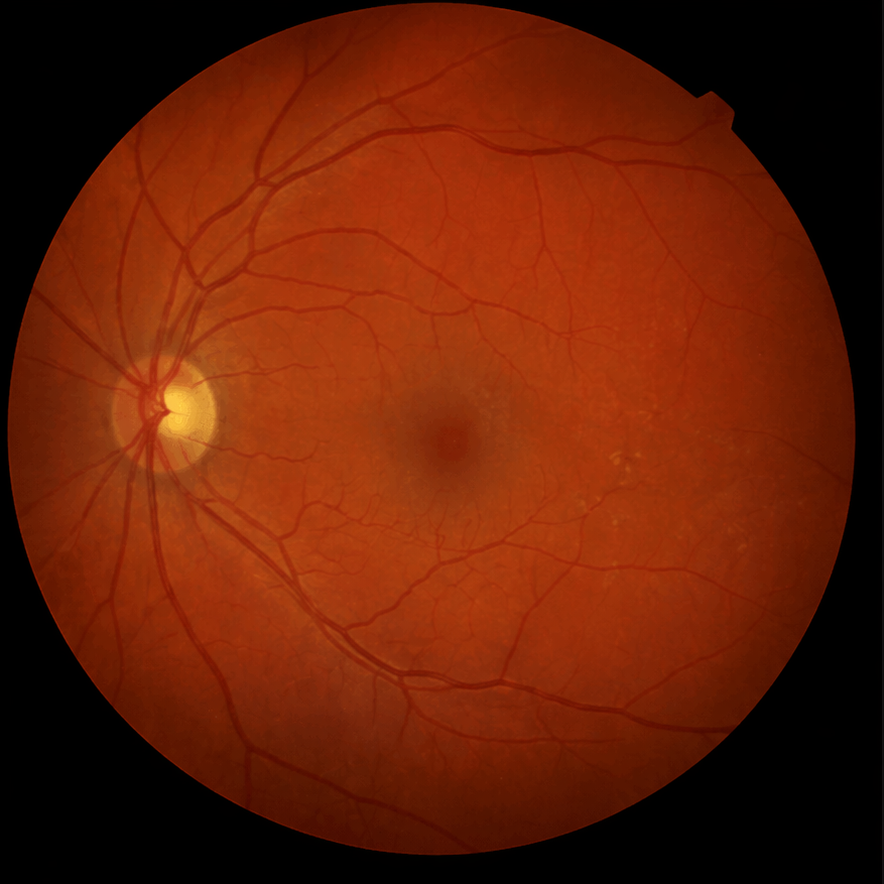
\includegraphics[width=\textwidth]{picture/retina_correcion/retina_normal_diabetes.png}
        \\[3pt]\small (a) Imagen original
    \end{minipage}
    \hfill
    \begin{minipage}[t]{0.31\textwidth}
        \centering
        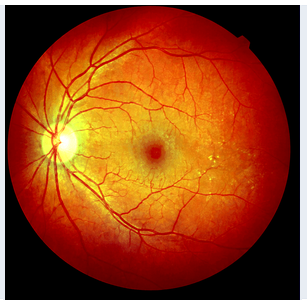
\includegraphics[width=\textwidth]{picture/retina_correcion/retina_normalizada.png}
        \\[3pt]\small (b) Imagen normalizada
    \end{minipage}
    \hfill
    \begin{minipage}[t]{0.31\textwidth}
        \centering
        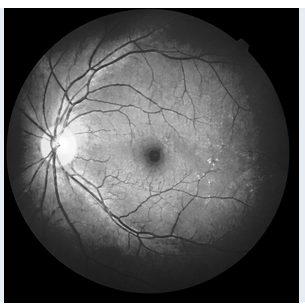
\includegraphics[width=\textwidth]{picture/retina_correcion/retina_comprimida_gris.png}
        \\[3pt]\small (c) Imagen en escala de grises
    \end{minipage}
    \caption{Comparación final entre la imagen original, la imagen normalizada y la imagen comprimida en escala de grises.}
    \label{fig:resultados_finales}
\end{figure}

Para complementar la comparación, la Figura~\ref{fig:exudados_marcados_gris_binaria} presenta lado a lado la imagen comprimida en escala de grises y la imagen binaria, ambas con los exudados señalados. Esta vista conjunta permite observar que los hallazgos detectados en la imagen normalizada también resultan visibles en la versión en escala de grises y se conservan en la representación binaria, lo que confirma que el procesamiento preserva los rasgos de mayor intensidad relacionados con los exudados a lo largo de las sucesivas etapas de simplificación.

\begin{figure}[H]
    \centering
    \begin{minipage}[t]{0.46\textwidth}
        \centering
        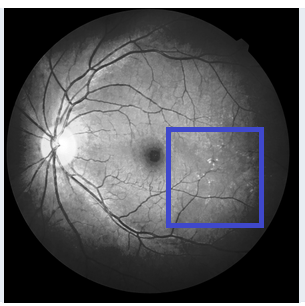
\includegraphics[width=\textwidth]{picture/retina_correcion/retina_comprimida_gris_exudados_marcados.png}
        \\[3pt]\small (a) Imagen comprimida en escala de grises
    \end{minipage}
    \hfill
    \begin{minipage}[t]{0.46\textwidth}
        \centering
        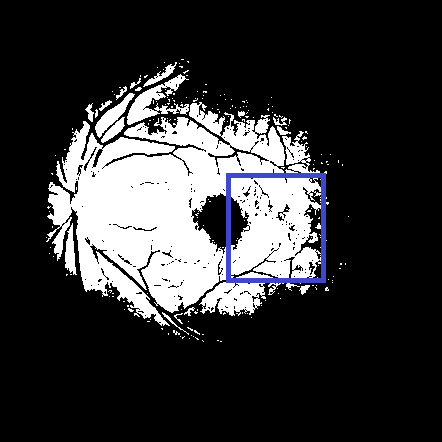
\includegraphics[width=\textwidth]{picture/retina_correcion/imagen_binaria_142_exudos.png}
        \\[3pt]\small (b) Imagen binaria con $T = 142$
    \end{minipage}
    \caption{Exudados identificados en la imagen comprimida en escala de grises y en la imagen binaria.}
    \label{fig:exudados_marcados_gris_binaria}
\end{figure}

En la imagen binaria, aunque la información visual queda reducida a únicamente dos valores, los exudados aparecen como pequeñas regiones identificables. La utilidad de esta observación radica en que, al ser una representación simplificada, la imagen binaria facilita la extracción automática de regiones de interés, permite aplicar operaciones morfológicas posteriores y puede servir como entrada directa para procesos de segmentación, conteo de estructuras o clasificación, sin necesidad de volver a procesar la información de color original.

Como observación adicional, al elevar el umbral de binarización a $T = 195$ se obtiene una segmentación más selectiva que permite identificar con mayor precisión las regiones de mayor intensidad asociadas a los exudados. Con este valor, la mayor parte del tejido retinal queda clasificada como negro, dejando en blanco únicamente las zonas con brillo elevado, lo que reduce el ruido visual y resalta con mayor claridad los posibles exudados respecto a los resultados obtenidos con umbrales más bajos.

\begin{figure}[H]
    \centering
    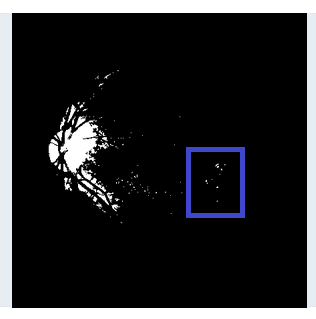
\includegraphics[width=0.55\textwidth]{picture/retina_correcion/binaria_195.png}
    \caption{Imagen binaria con $T = 195$: los exudados se destacan con mayor claridad al reducirse las regiones de brillo intermedio.}
    \label{fig:binaria_195}
\end{figure}

El procesamiento aplicado permitió mejorar la visualización de detalles que no eran evidentes en la imagen original, haciendo visibles los exudados presentes en el tejido retinal y facilitando su localización en la imagen normalizada, en la versión en escala de grises y en la representación binaria.

\subsection{Habilidades blandas empleadas en la práctica}
$\square$ Liderazgo \\
$\blacksquare$ Trabajo en equipo \\
$\square$ Comunicación asertiva \\
$\square$ La empatía \\
$\square$ Pensamiento crítico \\
$\square$ Flexibilidad \\
$\square$ La resolución de conflictos \\
$\square$ Adaptabilidad \\
$\blacksquare$ Responsabilidad \\

\subsection{Conclusiones}
\begin{enumerate}
    \item La normalización por canales mediante la técnica min-max permitió redistribuir las intensidades de la imagen original y mejorar el contraste del tejido retinal, logrando que los exudados, inicialmente imperceptibles a simple vista, resultaran visibles en la imagen procesada.

    \item El análisis por canales RGB evidenció que el canal verde aporta el mejor contraste para observar vasos, bordes y lesiones pequeñas, mientras que el canal rojo aporta información sobre la iluminación general y el canal azul ofrece un aporte reducido en este tipo de análisis.

    \item La conversión a escala de grises y la binarización permitieron simplificar la representación de la imagen y confirmar visualmente la ubicación de los exudados, mostrando que las zonas de mayor intensidad asociadas a estos hallazgos se conservan incluso al reducir la información de color.
\end{enumerate}

\subsection{Recomendaciones}
\begin{enumerate}
    \item Utilizar imágenes de retina con buena resolución y un formato homogéneo, ya que la calidad de la imagen de entrada influye directamente en la claridad de los resultados obtenidos tras la normalización, la compresión y la binarización.

    \item Ajustar de forma cuidadosa los rangos mínimo y máximo de cada canal, así como el tamaño de bloque y el umbral de binarización, teniendo en cuenta que valores inadecuados pueden eliminar detalles relevantes o introducir ruido en el resultado final.

    \item Interpretar los resultados del procesamiento siempre en comparación con la imagen original, evitando atribuir al procesamiento información que no estaba presente en la imagen y considerando que los hallazgos visuales obtenidos requieren validación posterior cuando se pretenda un uso más allá del análisis académico.
\end{enumerate}

\subsection{Referencias bibliográficas}
{
    \renewcommand{\refname}{}
    \vspace{-1.5em}

    \begin{thebibliography}{99}
        \bibitem{b1}
        R. C. Gonzalez and R. E. Woods, \textit{Digital Image Processing}, 4th ed. New York, NY, USA: Pearson, 2018.

        \bibitem{b2}
        A. K. Jain, \textit{Fundamentals of Digital Image Processing}. Englewood Cliffs, NJ, USA: Prentice Hall, 1989.

        \bibitem{b3}
        M. D. Abr\`amoff, M. K. Garvin, and M. Sonka, ``Retinal imaging and image analysis,'' \textit{IEEE Rev. Biomed. Eng.}, vol. 3, pp. 169--208, 2010.

        \bibitem{b4}
        J. Staal, M. D. Abr\`amoff, M. Niemeijer, M. A. Viergever, and B. van Ginneken, ``Ridge-based vessel segmentation in color images of the retina,'' \textit{IEEE Trans. Med. Imaging}, vol. 23, no. 4, pp. 501--509, Apr. 2004.
    \end{thebibliography}
}

\subsection{Anexos}

Como complemento al desarrollo principal, se presenta una aplicación adicional del flujo de procesamiento sobre una imagen distinta a la de retina, con el fin de evidenciar que el procedimiento definido resulta aplicable a otros casos de estudio. Se utilizó una fotografía del interior de una caverna, caracterizada por la presencia de zonas muy oscuras y regiones iluminadas, situación en la cual la normalización, la conversión a escala de grises y la binarización permiten resaltar detalles poco perceptibles en la imagen original.

\begin{figure}[H]
    \centering
    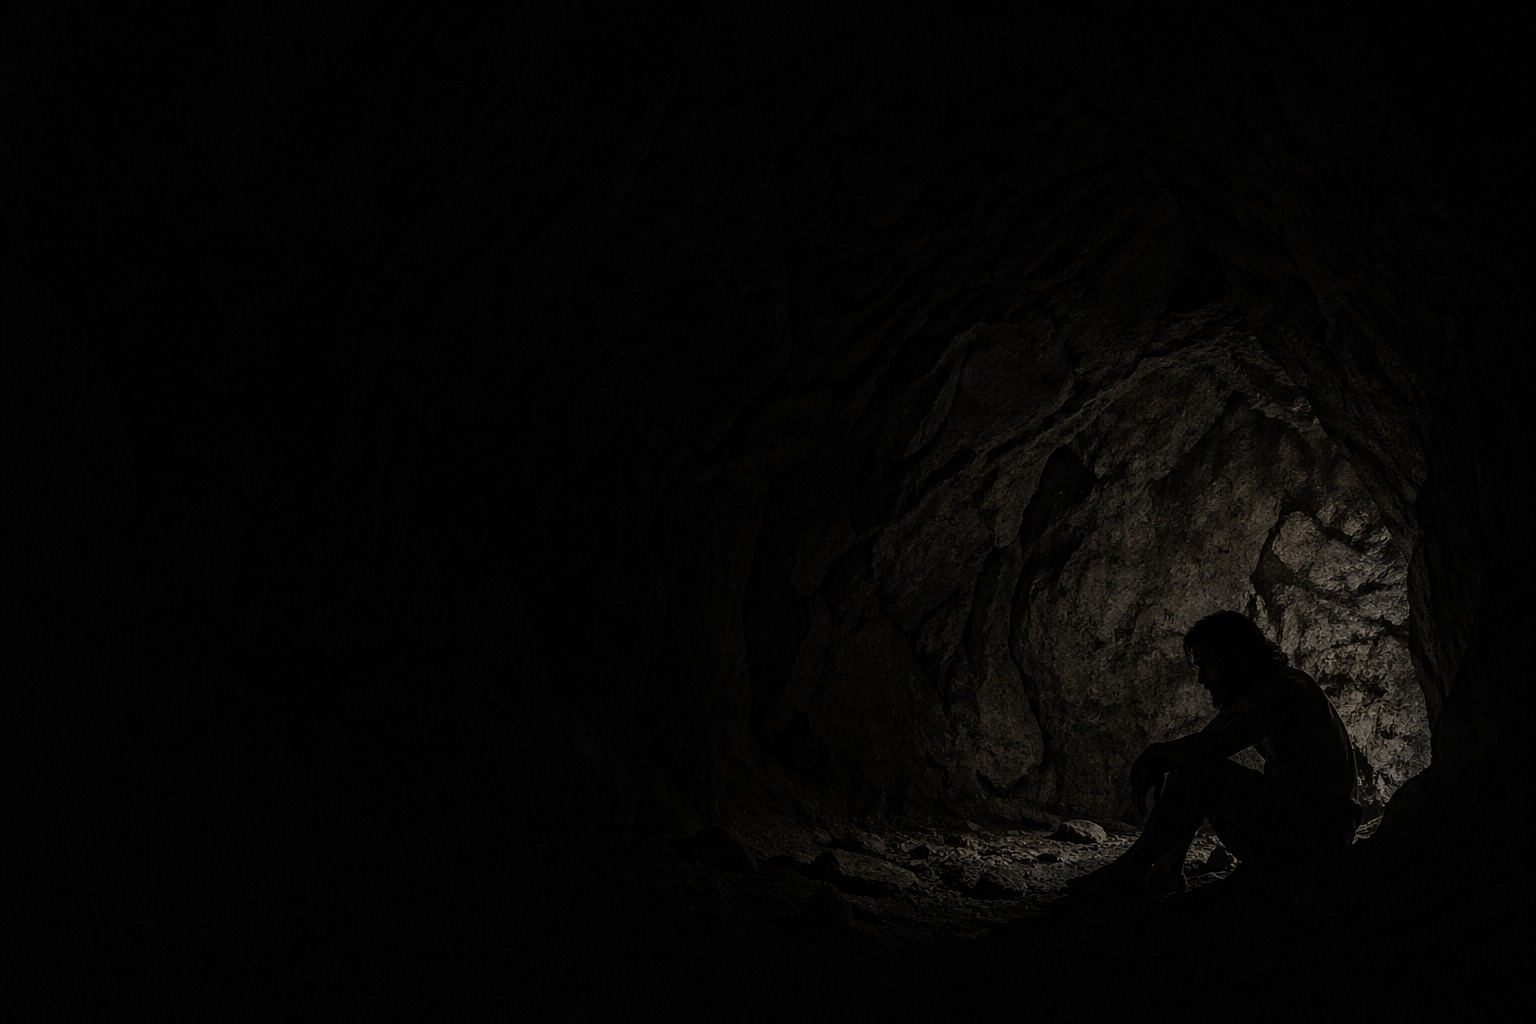
\includegraphics[width=0.65\textwidth]{picture/caverna/Anexo_otra_imagen_caverna_original.jpg}
    \caption{Imagen original empleada como caso adicional de procesamiento.}
    \label{fig:anexo_caverna_original}
\end{figure}

\begin{figure}[H]
    \centering
    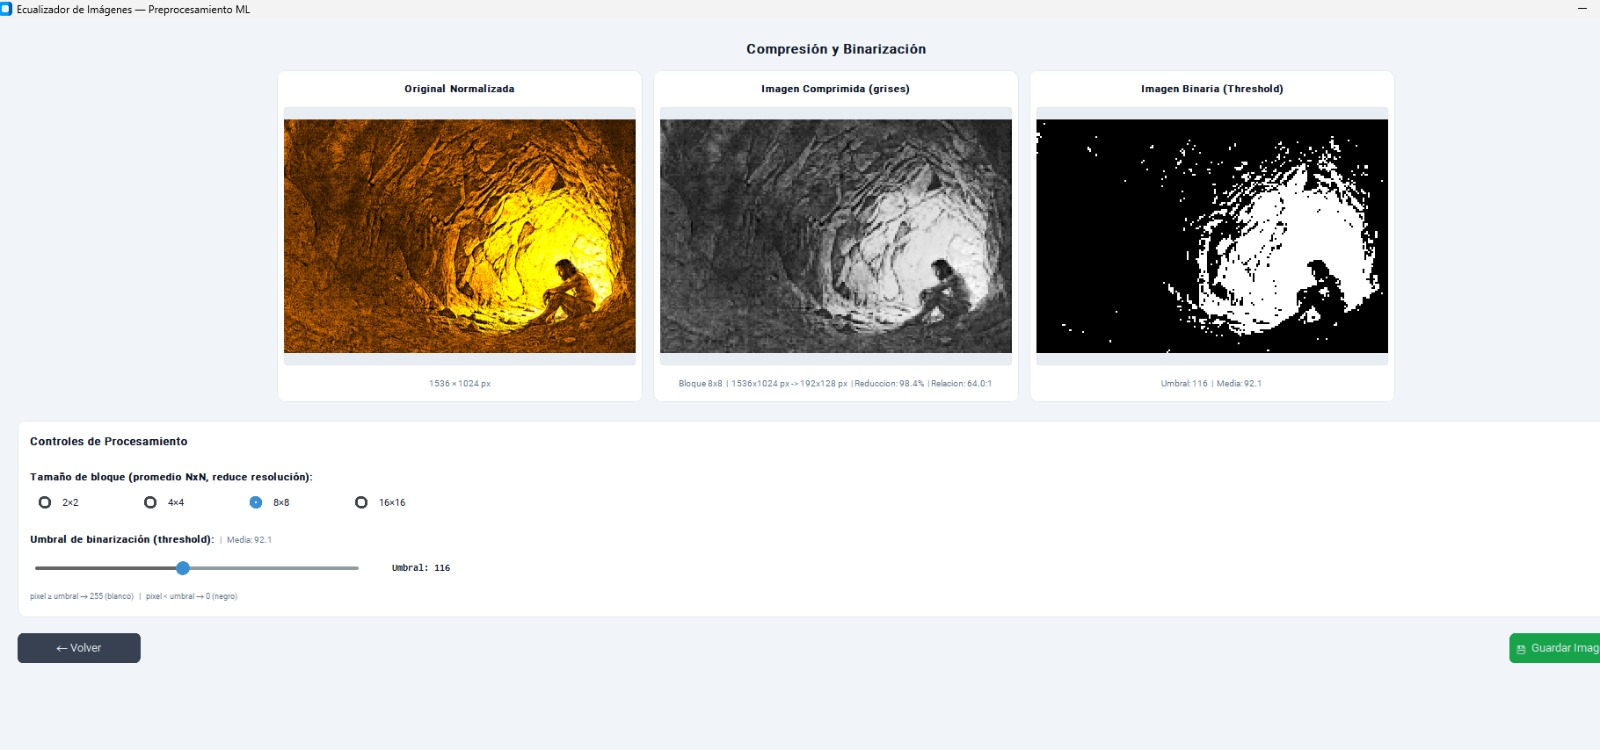
\includegraphics[width=0.95\textwidth]{picture/caverna/Anexo_otra_imagen_caverna_normalizada_gris_binario.jpg}
    \caption{Resultados obtenidos sobre la imagen adicional: versión normalizada, versión comprimida en escala de grises e imagen binaria.}
    \label{fig:anexo_caverna_resultados}
\end{figure}

\end{document}
